\%!TEX root=../document.tex

\section{Hardware-Aufbau}
\label{sec:Hardware-Aufbau}

asdfg \cite{brands11}

\begin{figure}[!htb]
	\centering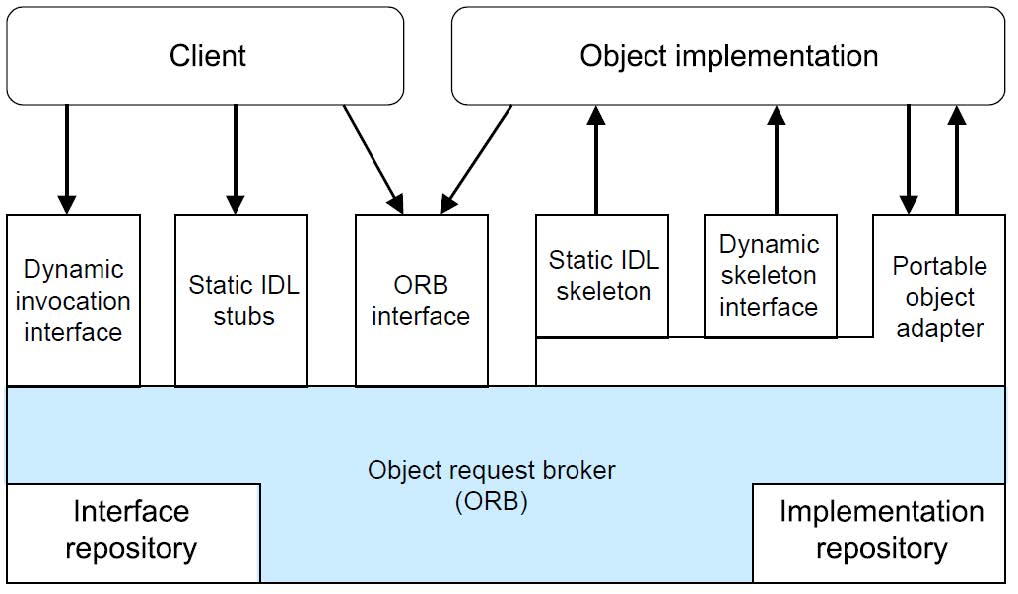
\includegraphics[width=0.8\textwidth]{images/corba.jpg}
	\caption{Ein Corba Bild}
	\label{corba}
\end{figure}

\begin{itemize}
    \item asdf
\end{itemize}


\subsection{Qubit}
\label{sec:Qubit}

\subsubsection{Schroedinger}

Schroedingers Katze ist die berühmteste Veranschaulichung eines grundlegenden Phänomens der Quantenmechanik. Genaugenommen ist es ein Versuchsaufbau, anhand dessen sich verschiedene Begriffe der Quantenmechanik leicht erklären lassen. Der Versuchsaufbau sieht folgendermaßen aus:

In einer Kiste befinden sich eine Katze und eine Ampulle mit einer Giftigen Substanz. Mit einer exakten Wahrscheinlichkeit von 50\% ist die Ampulle offen und die Katze bereits tot, mit einer genau gleich großen Wahrscheinlichkeit ist aber die Ampulle immer noch verschlossen und die Katze am Leben. Da wir nur die Außenseite der Kiste sehen und sie Schall und Geruchdicht ist, können wir nicht genau sagen, in welchem Zustand die Katze sich befindet. Es könnte also behauptet werden, dass sie gleichzeitig tot und lebendig ist.
Den Umstand, dass 2 (oft gegensätzliche) Zustände wahr sind, wird in der Quantenmechanik als Superposition bezeichnet. Eine Vorraussetzung für das erreichen einer Superposition ist die vollkommene Abschottung von der Außenwelt. 

Wenn nun die Kiste geöffnet wird und der Betrachter einen Blick ins innere der Kiste wirft, so erkennt er ziemlich schnell, ob die Katze tot oder lebendig ist. Einer der Beiden Zustände ist durch diese sogenannte Messung verloren gegangen.

\subsubsection{Definition}

Per Definition werden die Zustände eines Qubits in der Form \%alpha * |0> + \%beta * |1> angeschrieben.
\%alpha und \%beta werden "Amplituden" genannt, sind komplexe Zahlen und durch die Formel |\%alpha|^2 + |\%beta|^2 = 1 voneinander abhängig.
Anders als ein klassisches Bit, kann ein Qubit nicht gelesen, sondern muss gemessen werden, wobei die Superposition zerstört wird und anhand der Amplituden (die einen Anteil darstellen) folgendermaßen berechnet werden kann, mit welcher Wahrscheinlichkeit sich das Qubit in welchem Zustand befindet: P(|0>) = |\%alpha|^2, P(|1>) = |\%beta|^2

\subsubsection{Messung}

\subsubsection{Zust\"ande & Zustands\"anderungen}

\subsection{Register}
\label{sec:Register}

\subsubsection{Definition}
(formeln auf seite 28)

Ein Quantenregister besteht aus einer Reihe von 2 bis n Qubits und wird angeschrieben als <formel 1>
Zur Erklärung ist allerdings eine Beschränkung auf das Minumum von 2 Bits sinnvoll, deren Zustand folgendermaßen berechnet wird: <formel 2,3>
Der Zustand des Registers kann dann durch Ausmultiplizieren errechnet werden. <formel 4>

\subsubsection{Berechnung}

\subsubsection{Zust\"ande}

\subsubsection{begriffe "lokal" und "unit\"ar"}

\subsection{Gatter}
\label{sec:Gatter}

\subsubsection{CNOT}

CNOT bedeutet ausgesprochen "Controlled Not", was als "Kontrollierbare Negierungsschaltung" übersetzt werden kann.
Ein CNOT hat 2 Eingänge und 2 Ausgänge, wobei der zweite Ausgang den invertierten Wert von 1 ausgibt wird, wenn der erste Eingang auf 1 gesetzt ist.

\subsection{Architektur}
\label{sec:Architektur}

\subsubsection{Anforderungen}

Definition von David Deutsch 1985:
Ein Quantencomputer besteht aus einer Reihe von Quantenbits,
1. die in einen Anfangszustand versetzt werden k\"onnen,
2. die Information robust speichern,
3. auf die (universelle) Quantengatter anwendbar sind und
4. die gemessen werden k\"onnen.

\subsubsection{(De)koh\"arenz}

Kohärenz bedeutet Zusammenhängend. Dekohärenz ist ein Phänomen der Quantenphysik, das Kohärenzeigenschaften von Systemen kurzzeitig außer Kraft setzt. Dekohärenzeffekte treten auf, wenn ein geschlossenes System geöffnet wird und mit der Umwelt in Wechselwirkung treten kann, wobei die Zustände beider Systeme irreversibel verändert werden.
Im Beispiel mit der Katze, wäre es eine Tote oder lebende Katze, und der Betrachter, der nun weiß, ob die Katze tot oder lebendig ist.

\subsubsection{Photonen}

Die Physiker Ludwig Mach und Ludwig Zehnder entwickelten unabhängig voneinander beide den selben Versuchsaufbau, der heutzutage Mach-Zender-Inferometer genannt wird. Er besteht aus 4 Spiegeln, wovon 2 halbdurchlässig sind, 2 Messgeräten und einem Streifen Papier.

Wenn ein Lichtstrahl in den Aufbau geschickt wird, so wird er über den ersten Spiegel, der halbdurchlässig ist, geteilt in eine gerade und eine um 90° abgelenkte Bahn gelenkt. Nach einem gewissen Abstand befindet sich auf jeder Bahn einer der "normalen" Spiegel, wodurch das Licht jeweils um 90° gelenkt wird und sich die beiden dann an einer Stelle kreuzen, an der der zweite halbdurchlässige Spiegel montiert wird. In eine Bahn wird ein Blatt Papier gehalten. Durch den halbdurchlässigen Spiegel kommt bei beiden Messgeräten gleich viel Licht an. Wird das Blatt Papier entfernt, so kommt es auf einer Bahn zu konstruktiven überlagerungen zwischen dem letzten Spiegel und dem Messgerät, wodurch bei diesem kein Licht ankommt.

Wenn anstelle eines Lichtstrahles nur einzelne Photonen verwendet werden, zeigt sich der selbe Effekt, obwohl eigentlich keines der Photonen wissen kann, ob der Papierstreifen im Weg ist oder nicht. Und hier kommt wieder die Quantenphysik als Erklärung zum einsatz, da ein Teilchen, wie wir schon wissen, solange es nicht beobachtet wird, in mehreren Zuständen gleichzeitig sein kann. Es kann sich also auf beiden Bahnen gleichzeitig bewegen, bis es gemessen wird, wodurch die Superposition zerstört wird und es nur bei einem Messgerät ankommen kann.

\subsubsection{Kernspinresonanz}

Kernspinresonanz ist der Name für einen phyiskalischen Effekt der in Form von Wechselwirkung zwischen Atomkernen und Magnetfeldern auftritt. Der Spin eines Moleküls kann durch Magnetfelder ausgerichtet werden, was ausgenutzt wird, um Quantenbits abzubilden und zu speichern. Durch unterschiedliche chemische Eigenschaften der Umgebung kann jedes Bit einzeln angesprochen werden. Mithilfe eines Hauptmagnetfeldes kann man die Zustande definieren, zum Beispiel als: gleiche Ausrichtung = |0>, im rechten Winkel = |1>;

\subsubsection{Ionenfallen}

Ionenfallen sind dazu da, um elektrisch geladene Moleküle oder Atome durch Magnetfelder an ein und der selben Position zu halten, wodurch mit einem gefangenen Ion bis zu 2 Quantenbits abgebildet werden können. Die abstände zwischen mehreren Ionen liegen im Mikrometerbereich, können durch einen Laser einzeln adressiert werden, aber müssen Temperaturmäßig nahe dem Absoluten gehalten werden um sich nicht gegenseitig abzustoßen.

\section{Interkommunikation}
\label{sec:Interkommunikation}


\subsection{Quantennetzwerke/Kanäle}
\label{sec:Quantennetzwerke/Kanale}

\subsubsection{Generelles Schema eines Telekommunikationssystems}

\subsubsection{Klassische- vs. Quanten-Kommunikationskan\"ale}

\subsubsection{Photonz\"ahlung}


\subsection{Quantenteleportation}
\label{sec:Quantenteleportation}






